\documentclass[a4paper]{article}
\usepackage[a4paper,top=1cm,bottom=2cm,left=2cm,right=2cm,marginparwidth=1.75cm]{geometry}
\usepackage{amsmath}
\usepackage{graphicx}
\usepackage{amssymb}
\usepackage[colorlinks=true, allcolors=blue]{hyperref}
\usepackage{mathtools} 
\usepackage{extarrows} 
\usepackage[belowskip=-8pt,aboveskip=5pt]{caption}

\setlength{\intextsep}{10pt plus 2pt minus 2pt}
%\titlespacing\section{0pt}{6pt plus 0pt minus 0pt}{11pt plus 0pt minus 2pt}
% \title{\textbf{EN2550 - Fundamentals of Image Processing and Machine Vision}\\
% Assignment 02}
\author{Tharindu O.K.D.\\19062R}
\begin{document}
%\maketitle
\begin{center}
  \textbf{Tharindu O.K.D.\\190622R}\\
  \href{https://github.com/dakshinatharindu/Image-Processing/blob/main/Assignment-02/190622R_a02.ipynb}{GitHub Repository (click here)} 
\end{center}

\section*{Question 01}
\begin{figure}[!htb]
    \centering
    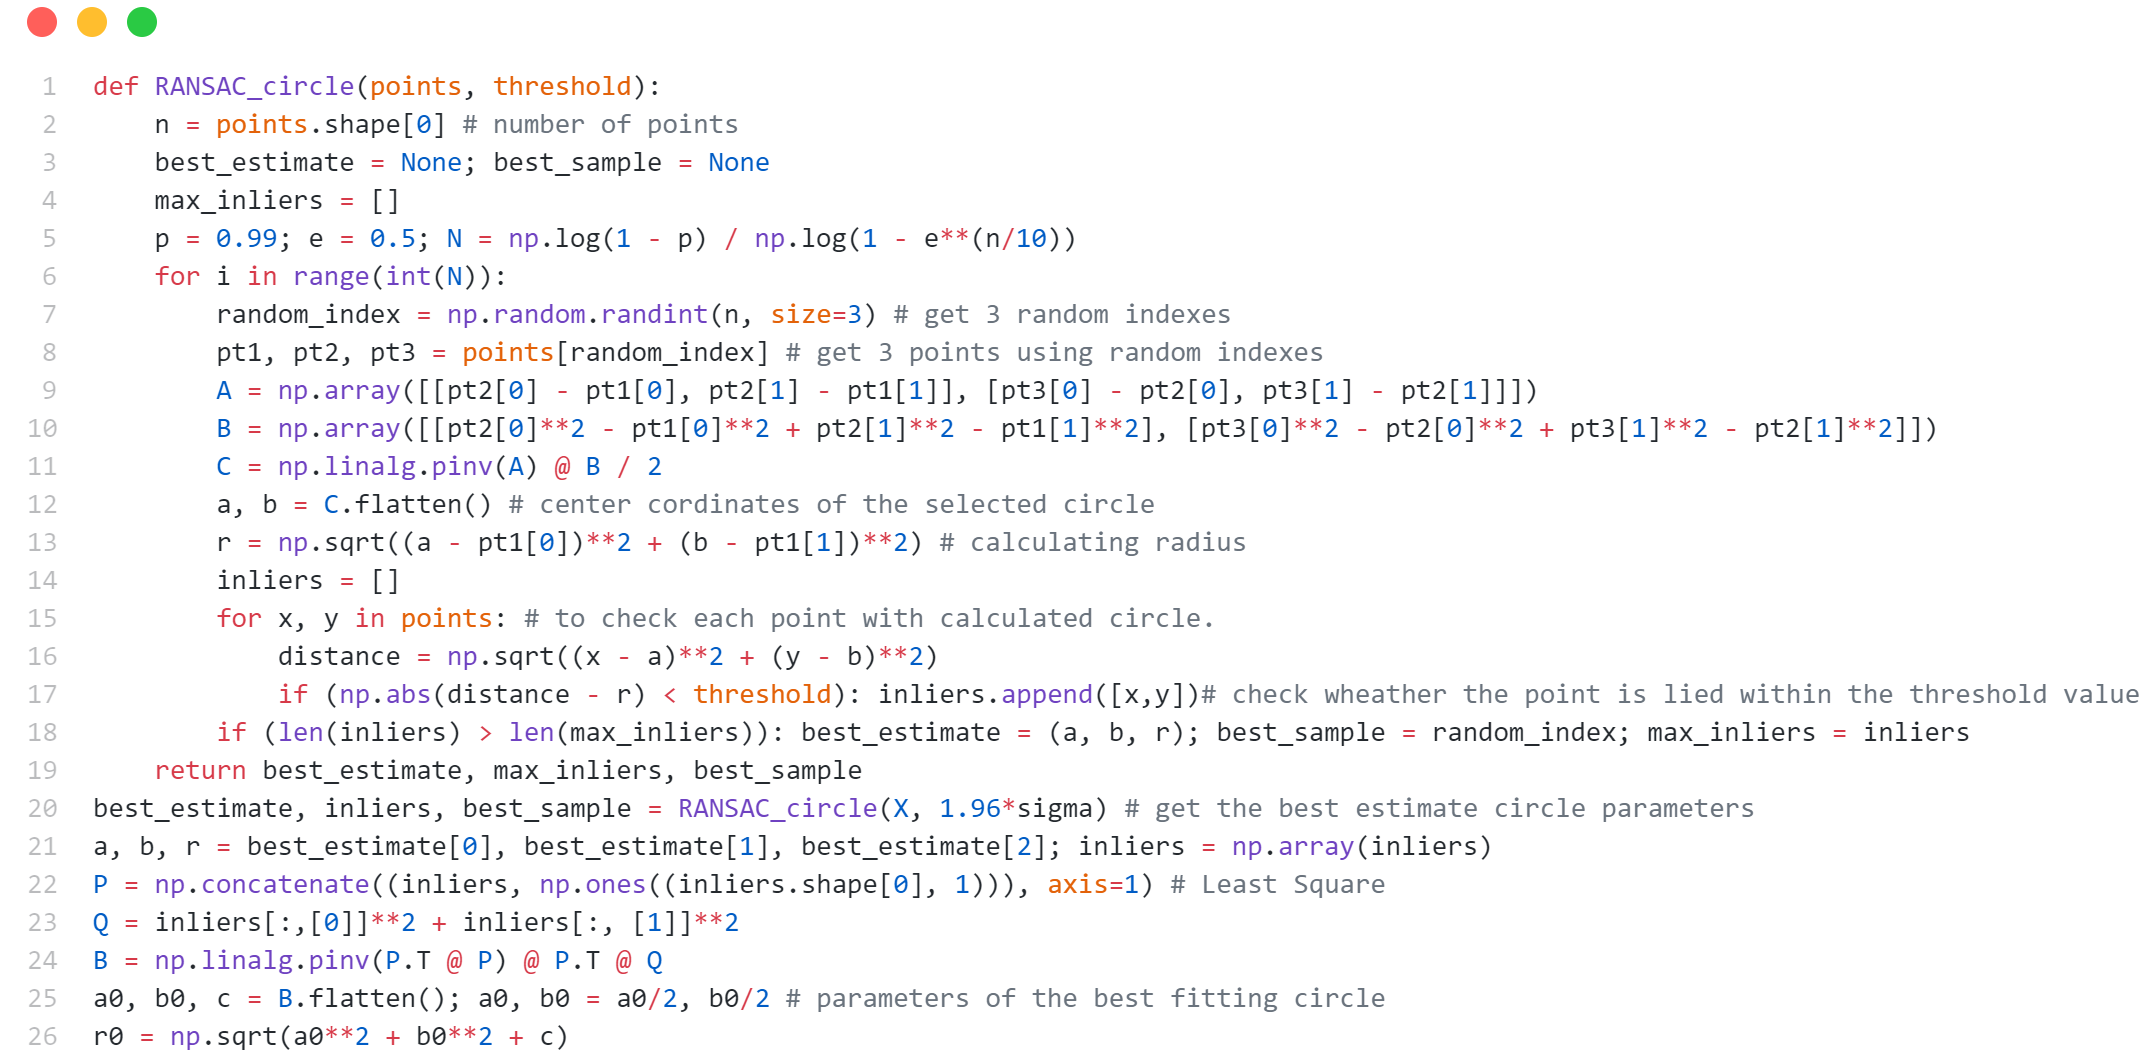
\includegraphics[width=\textwidth]{images/ransac_circle.png}
    \caption{Question 01 Code}
    \label{ransac_circle}
\end{figure}
Our objective for this is to robustly fit a circle to our point set.
 This can be done using the RANSAC algorithm to find the best inlier
  set and then fit a circle to this inlier set.
   Figure \ref{ransac_circle} shows the code snipped
    of the RANSAC function. Approach of this method is shown below.
\begin{enumerate}
  \itemsep0em 
  \item First, we calculate the number of iterations $N$ required to get a better estimation. We choose $N$ 
  so that, with probability $p$, at least one random sample is free from outliers.
  It is given by, $N=\frac{\log{(1-p)}}{\log{(1-(1-e)^n)}}$. Here $e$ is outlier
  ratio and $n$ is a number of points. Here I took $e=0.5$ and $p=0.99$ so 
  that 50\% of points will fall into inliers with a 99\% probability.
  \item We randomly select 3 points from the given data set. Then we calculate the fitting
   circle using the cartesian equation of the circle $(x-a)^2+(y-b)^2=r^2$. Substituting
    3 point coordinates and putting it into matrix form, we get
   \begin{align*}
     \begin{pmatrix}
       x_2-x_1 & y_2-y_1\\
       x_3-x_2 & y_3-y_2
     \end{pmatrix}
     \begin{pmatrix}
       2a\\
       2b
     \end{pmatrix}&=
     \begin{pmatrix}
      x_2^2-x_1^2 & y_2^2-y_1^2\\
      x_3^2-x_2^2 & y_3^2-y_2^2
    \end{pmatrix}
   \end{align*}
   Then we can find center coordinates $(a, b)$ and radius$(r)$ by solving above matrix equation.
   \item Then determine the inlier set 
   $=\{(x_i,y_i)\in points \text{ s.t }|\sqrt{(x_i-a)^2+(y_i-b)^2}-r|<threshold\}$
   \item If $|inliers|>|max\_inliers|$, we select it as the best estimate. Go to step 2
   until iterate N times.
  \end{enumerate}
First, we get the parameters of the best fitting circle using the above 
$RANSAC\_circle$ function. Since the sample noise is distributed as zero-mean
 Gaussian, we pass the threshold value as $1.96\sigma$ so that will give
  a $\approx95\%$ probability of capturing all inliers. After
   finding the best inliers, we find the best fitting circle for
    those inliers using the Least Square approach as follows.
    \begin{align*}
      \begin{pmatrix}
        x_1 & y_1 & 1\\
        x_2 & y_2 & 1\\
        \vdots & \vdots & \vdots\\
        x_n & y_n & 1\\
      \end{pmatrix}
      \begin{pmatrix}
        2a_0 \\ 2b_0 \\ c
      \end{pmatrix}&=
      \begin{pmatrix}
        x_1^2 & y_1^2\\
        x_2^2 & y_2^2\\
        \vdots & \vdots \\
        x_n^2 & y_n^2\\
      \end{pmatrix}\\
      PB&=Q\\
      B&=(P^T P)^{-1}P^T Q
    \end{align*}
    Using the B matrix, we can find
     $a_0, b_0$, and $r_0$ which are the parameters of the best-fitting
      circle.
\begin{figure}[!htb]
  \centering
  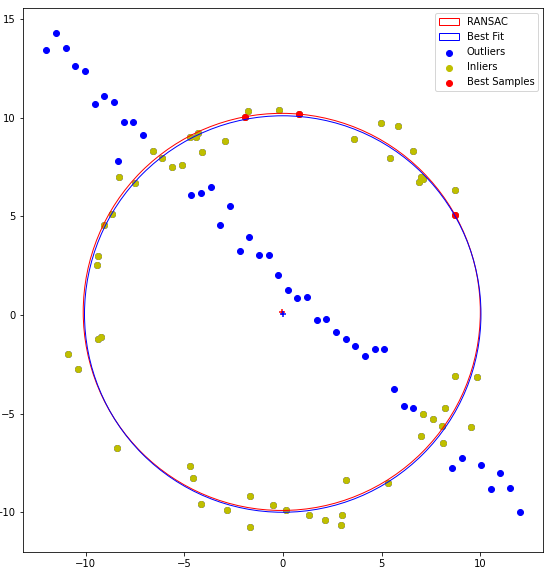
\includegraphics[width=0.4\textwidth]{images/ransac.png}
  \caption{Output}
  \label{ransac}
\end{figure}
\newpage
\section*{Question 02}


\begin{figure}[!htb]
  \centering
  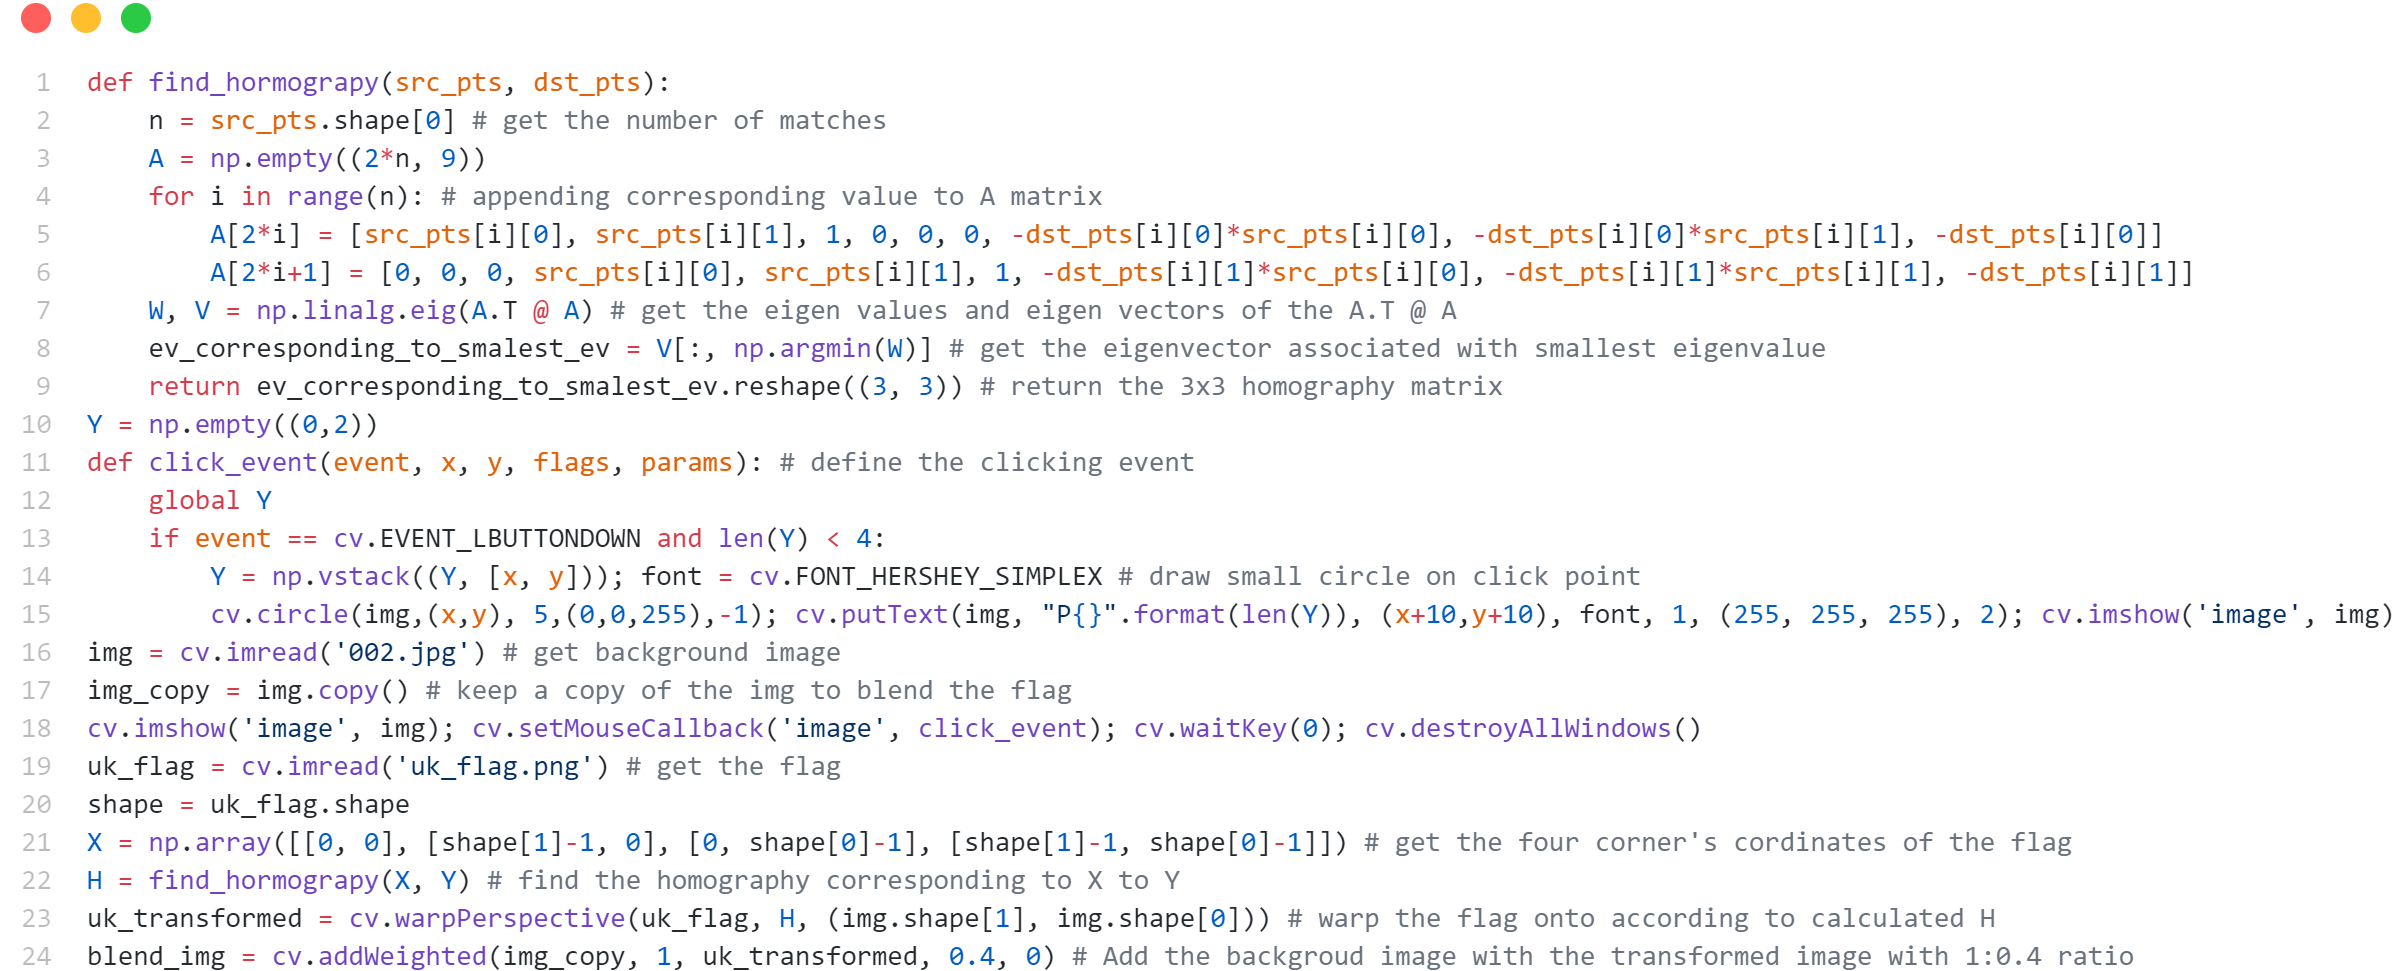
\includegraphics[width=\textwidth]{images/q2code.png}
  \caption{Question 02 Code}
  \label{q2code}
\end{figure}
The objective of this question is to superimpose the flag into the given background image.
\begin{enumerate}
  \itemsep0em 
  \item First, we find the coordinates of the selected points ($Y$) using
   mousing clicking and find the coordinates of the four corners($X$) of
    the flag. Then we feed these source points ($X$) and destination points
     ($Y$) to the $find\_homography$ function as shown in Figure \ref{q2code}.
  \item Although, we only need four correspondences to find the
   homography matrix, in this function, if we give more than four
    points it will calculate the homography matrix using the least
     square approach  ($\because$ this will be required for question 03). This
      will not be a problem because if we give the exact four
       correspondences, it will return the exact homography matrix.
        In the $find\_homography$ function,
   we put each coordinate into matrix form as shown below.
   \begin{align*}
     \begin{pmatrix}
       \vdots & \vdots & \vdots & \vdots & \vdots & \vdots & \vdots & \vdots & \vdots\\
       x_s^{(i)} & y_s^{(i)} & 1 & 0 & 0 & 0 &-x_d^{(i)}x_s^{(i)} &-x_d^{(i)}y_s^{(i)} & x_d^{(i)}\\
       0 & 0 & 0 & x_s^{(i)} & y_s^{(i)} & 1 & -y_d^{(i)}x_s^{(i)} &-y_d^{(i)}y_s^{(i)} & y_d^{(i)}\\
       \vdots & \vdots & \vdots & \vdots & \vdots & \vdots & \vdots & \vdots & \vdots
     \end{pmatrix}
     \begin{pmatrix}
       h_{11} \\ h_{12} \\h_{13} \\ h_{21} \\ h_{22} \\ h_{23} \\ h_{31} \\ h_{32} \\ h_{33}
     \end{pmatrix}&=
     \begin{pmatrix}
       \vdots \\ 0 \\ \vdots
     \end{pmatrix}\\
   \end{align*}
   $$Ah=0$$
   Since $H$ is defined up to a scale value, we can solve
    this as a Constrained Least
     Square problem. i.e. $h$ is 
     the eigenvector associated with the smallest eigenvalue
      of the matrix $A^TA$. Then we can find the $H$ matrix using $h$ vector.
    \item After finding the homography matrix, we can use the
     OpenCV warpPerspective
      method to warp the flag into selected points.
       To blend the two images, I have used the OpenCV
        addWeighted method which will add the two images with
         a given ratio.
    \end{enumerate}
Figure \ref{q2} shows selected points in the order and the resulting
     image for the UK flag and Sri Lanka flag.


\begin{figure}[!htb]
  \centering
  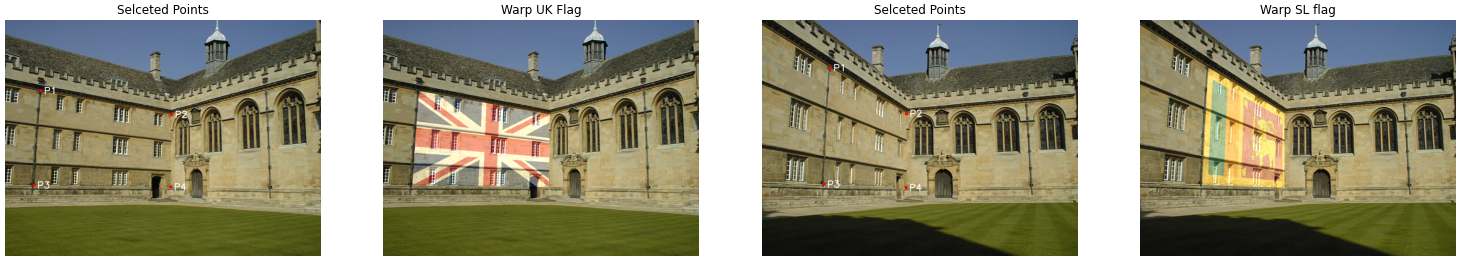
\includegraphics[width=\textwidth]{images/q22.png}
  \caption{Output}
  \label{q2}
\end{figure}


\section*{Question 03}

\begin{figure}[!htb]
  \centering
  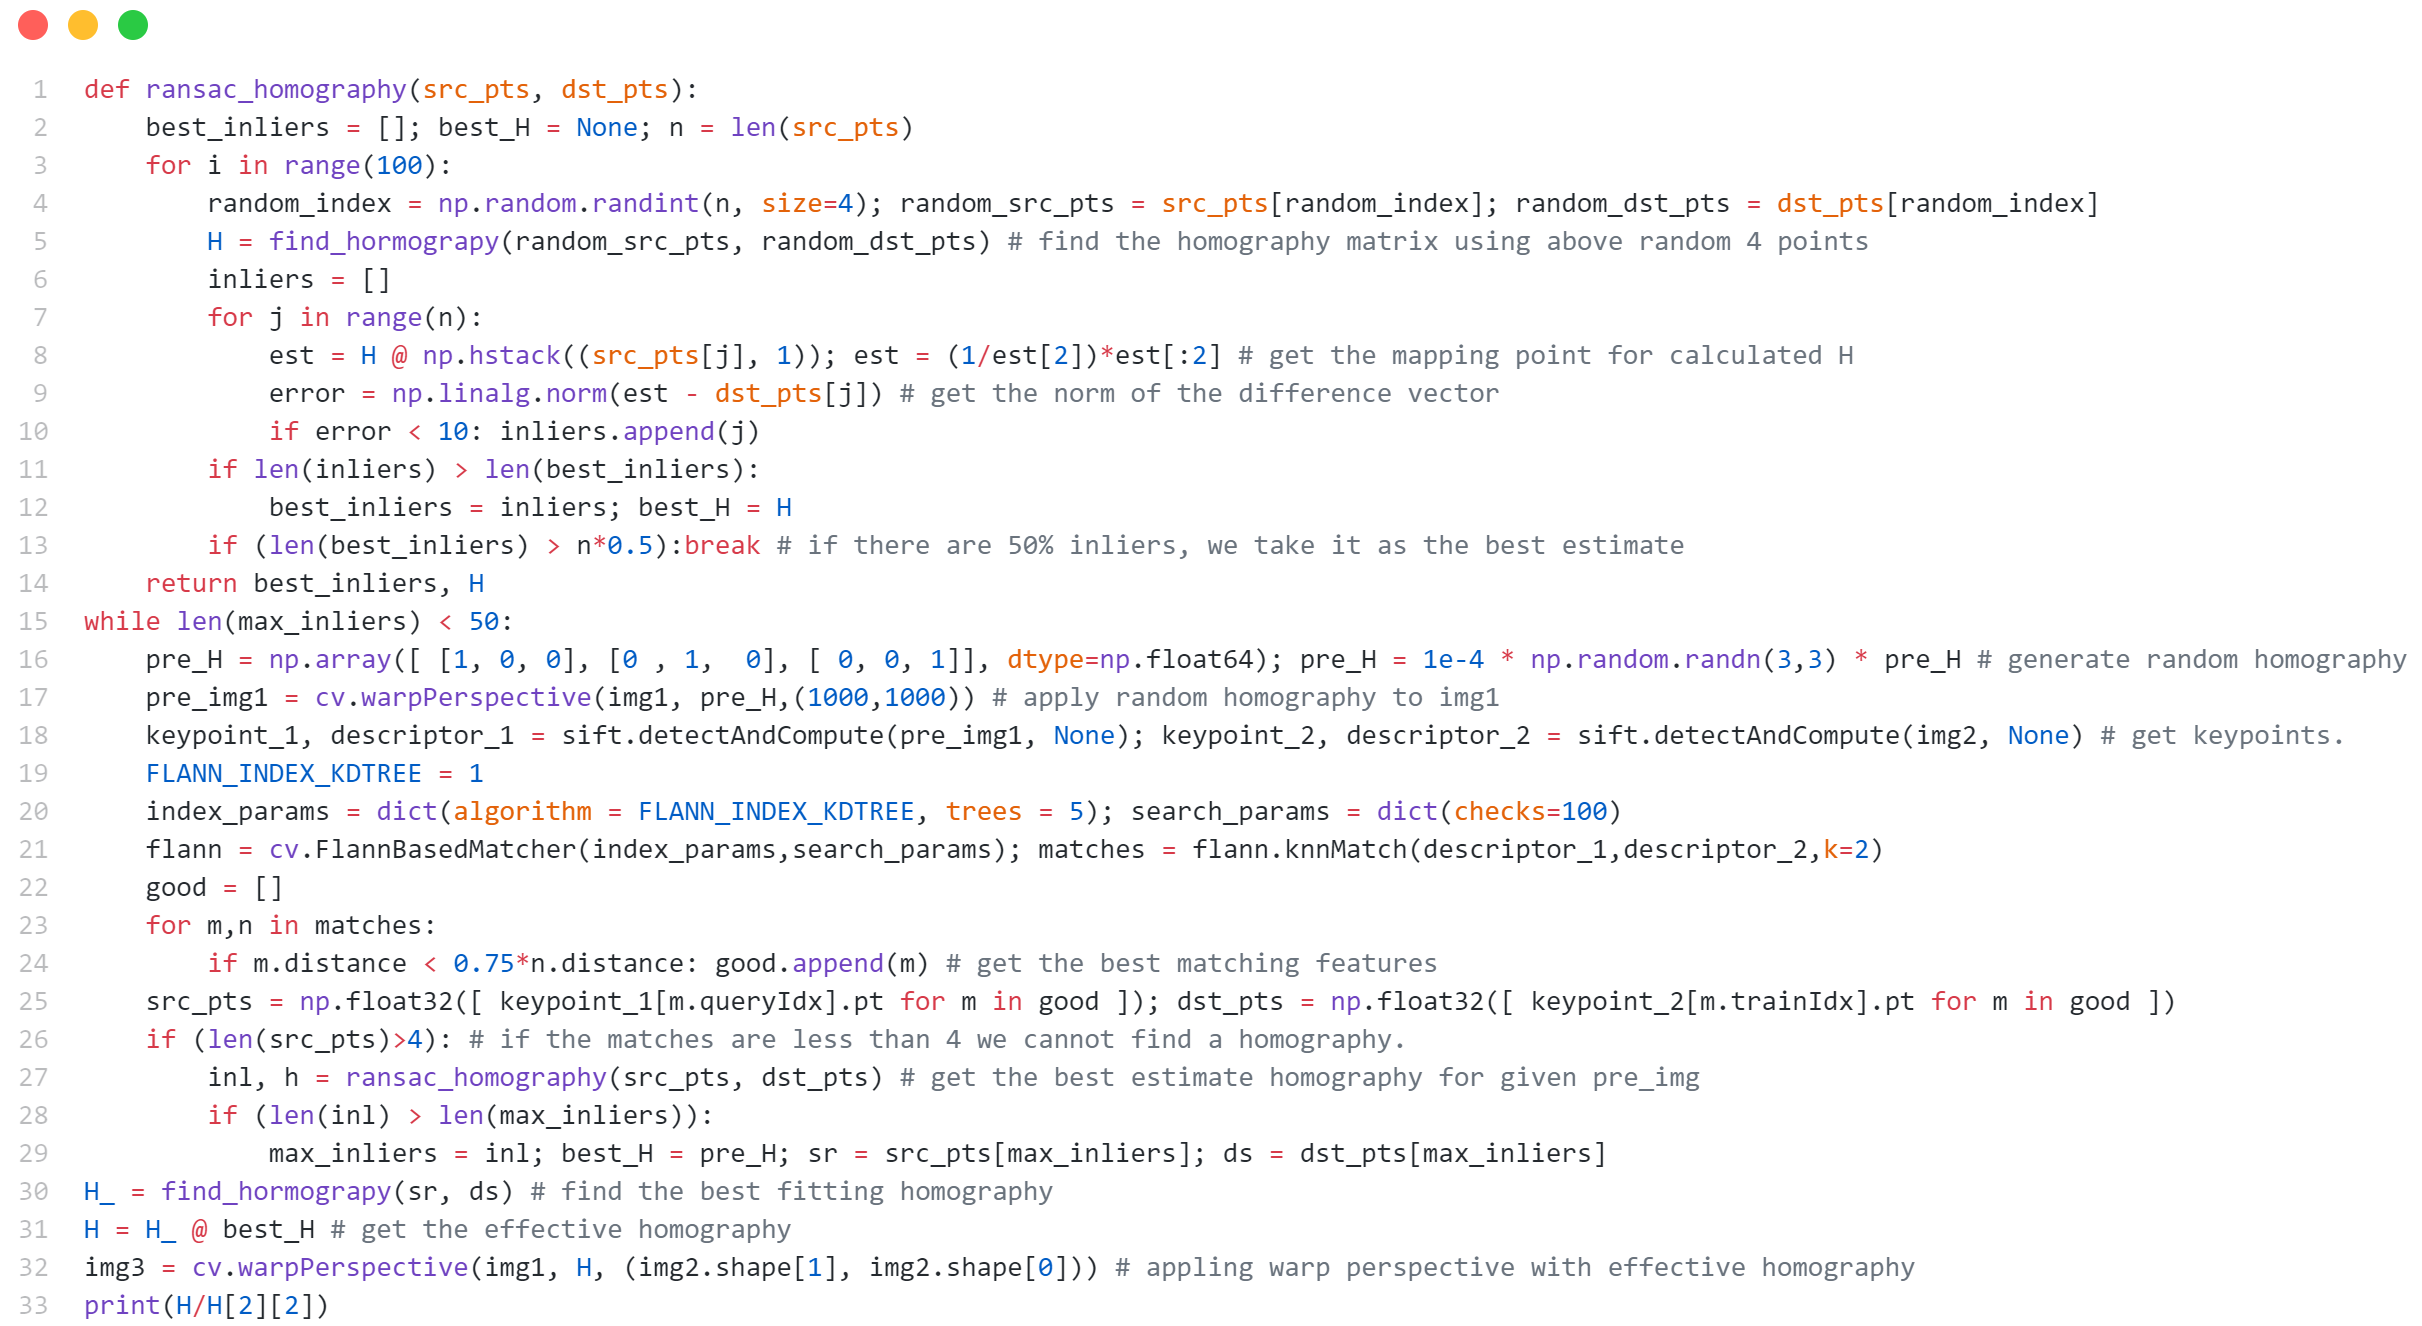
\includegraphics[width=\textwidth]{images/q3code.png}
  \caption{Code}
  \label{q3code}
\end{figure}
\begin{figure}[!htb]
  \centering
  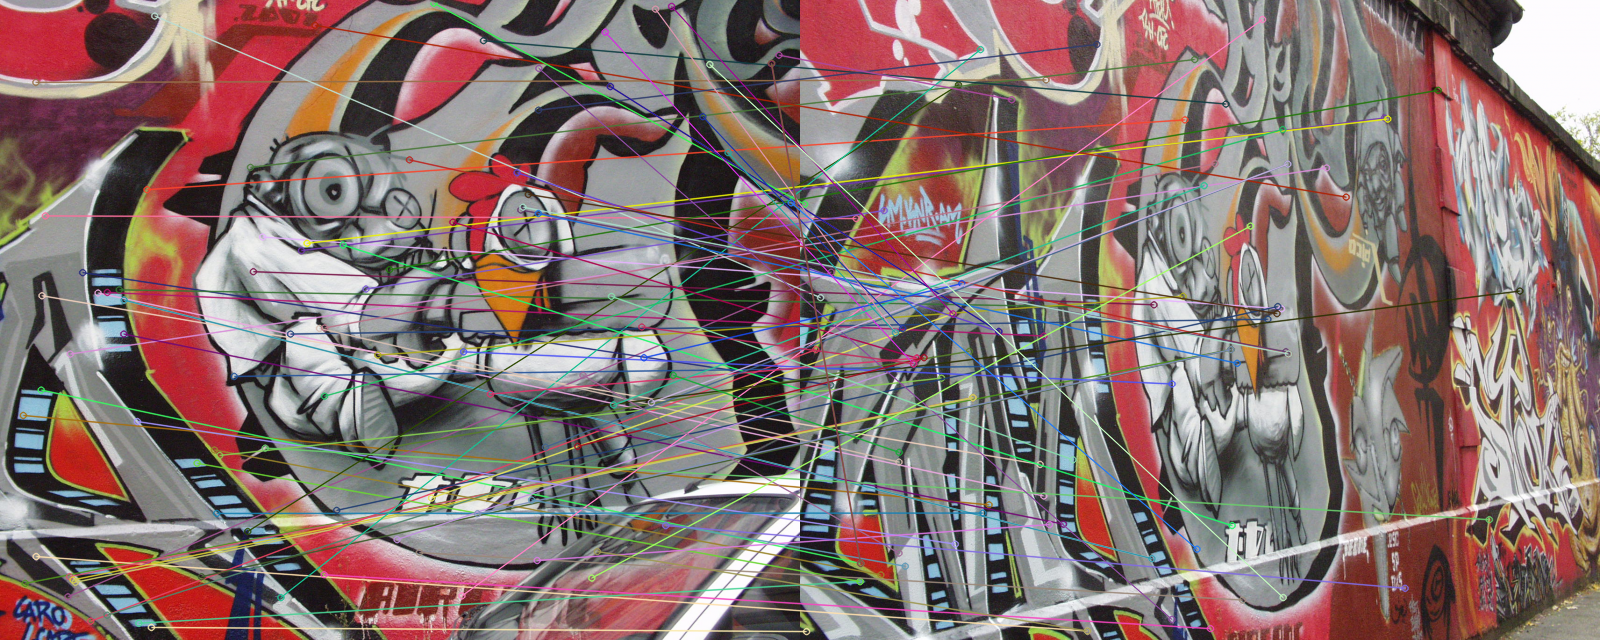
\includegraphics[width=0.65\textwidth]{images/stif.png}
  \caption{Match SIFT Features}
  \label{sift}
\end{figure}
I have used a FLANN-based matcher to match SIFT features rather
 than using a Brutal-Force matcher because it gives very accurate
  and more matches. You can see that in Figure \ref{sift},  even though we
   used the FLANN-based matcher, we only get a fewer number of SIFT
    matches and lots of them are incorrect. This is happen because
     img5 is taken more parallel to the wall. Therefore, the img5
      is more compact in the horizontal direction than img1.
       Therefore, lots of features are missed and incorrect.
        So, if we directly calculate the homography using these 
        matches, we will get a wrong homography matrix.
  
To overcome this problem, I have used the following method.
\begin{enumerate}
  \itemsep0em 
  \item First I apply a random pre-homography
   transformation to img1. Since we do not need
    any translation, I force it to be zero and
     also force vector $v$ of the homography matrix to be zero.
  \item Apply the warp perspective transformation to img1 with
   the above random pre-homography transformation. Then match
    the SIFT features of the resultant pre-transformed image 
    and img5.
  \item Then apply the ransac\_homography function with these matching
   points. It first randomly picks 4 correspondences and finds the
    corresponding homography matrix using the find\_homography
     function defined in question 02. Then apply the homography
      to each source point and calculate the vector norm with
       the destination point. If the norm value is less than
        the threshold value, we append this to the inlier set.
         After iterating 100 times, it returns the best homography
          matrix with inliers. I constrained the iteration time to 
          100 because some random warp perspective may not have
           any matches.
  \item Repeat the above 3 steps until we find the pre-homography
   which gives more than 50 inliers. Then calculate the best fitting
    homography using the find\_homography function 
    (As mentioned in question 02, this function is capable
     of finding homography using the least square method).
  \item After finding the best homography
   for the pre-transformed image to img5,
    we can calculate the effective homography using
     the above pre-homography and calculated homography.
     $$img1 \xrightarrow{H_{21}} pre\_transformed\_image \xrightarrow{H_{32}} img5$$
     $$img1 \xrightarrow{H_{31}=H_{32}H_{21}}  img5$$
\end{enumerate}
\begin{align*}
  calculatedHomography&=
  \begin{pmatrix}
     6.14979996e-01&  5.93985823e-02 & 2.21696291e+02\\
     2.15344442e-01  &1.15345300e+00 &-2.28382302e+01\\
  4.74622983e-04 &-4.59124680e-05&  1.00000000e+00
  \end{pmatrix} \\ givenHomography&=
  \begin{pmatrix}
    6.2544644e-01 &  5.7759174e-02 &  2.2201217e+02\\
    2.2240536e-01 &  1.1652147e+00 & -2.5605611e+01\\
    4.9212545e-04 & -3.6542424e-05 &  1.0000000e+00
  \end{pmatrix}
\end{align*}
As you can see, calculated homography and given homography are almost 
the same. Therefore we can confirm that this method performs well
rather than directly matching SIFT features. After finding the warp
 perspective image, I have used 3 methods to blend the image. First, 
 I directly add the resultant image to img5 with 50-50\% weight. 
 As you can see the common area is more highlighted. In the second 
 method, I cut the perspective of the img1 from img5 and then add 
 the two. This gives a better result but we can still see the seams 
 of the joining lines. Lastly, rather than directly cutting the 
 perspective, I applied a distance transformed mask to the resultant 
 image and then add the two images. You can see this gives a better 
 result than the other two methods.







\begin{figure}[!htb]
  \centering
  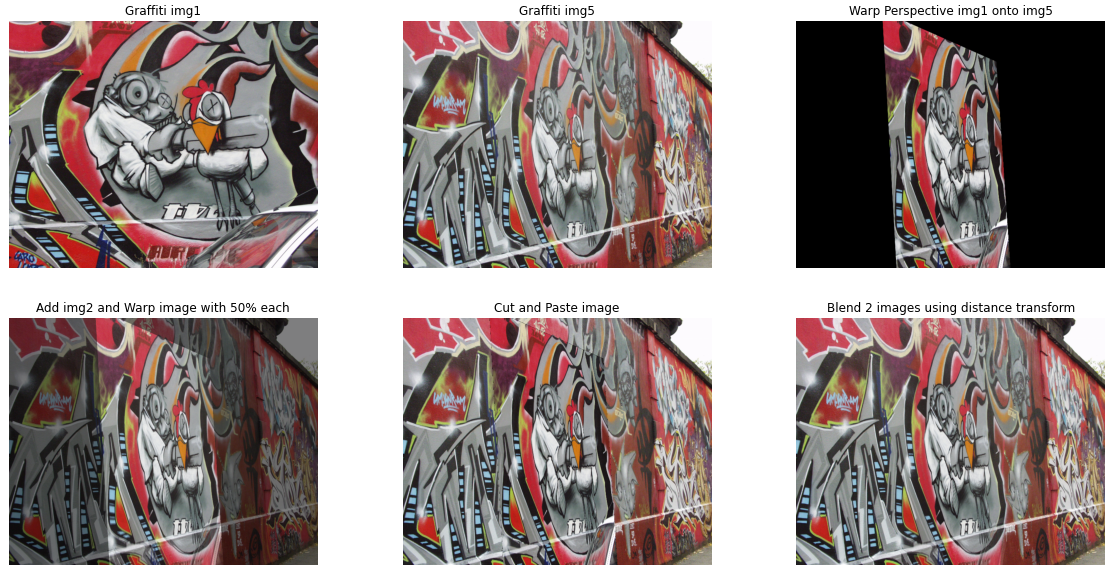
\includegraphics[width=\textwidth]{images/q3.png}
  \caption{Output}
  \label{q3}
\end{figure}
\end{document}
